\section{Esercizio 15}
\textit{\textbf{Descrizione:} Scrivere un programma che implementi efficientemente il calcolo del polinomio interpolante di Hermite su un insieme di ascisse distinte.}\newline
\noindent\emph{Soluzione: }\newline

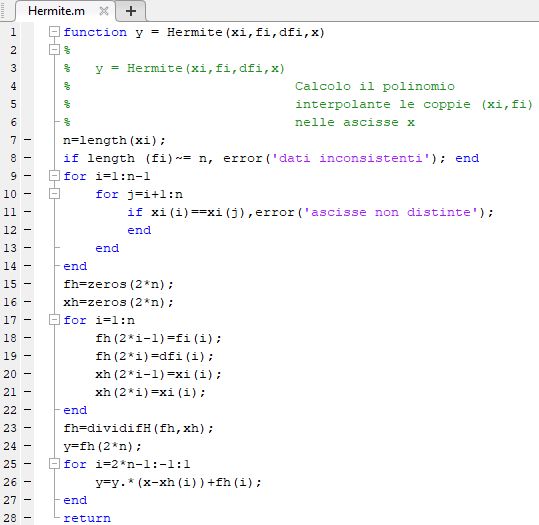
\includegraphics[width=1.3\linewidth]{img/Hermite.png}
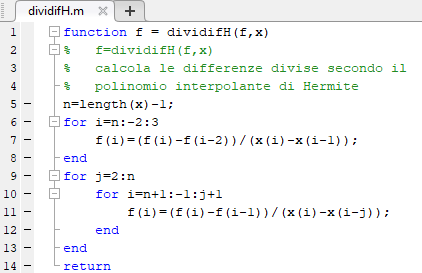
\includegraphics[width=1.3\linewidth]{img/dividifH.png}\newpage